\chapter{الاحتراق: أنواع الوقود ونواتجه وغازات الدفيئة}\label{ch:g8:combustion-and-fuels}

تنام أسرة في شقة انسدّت مدخنة سخّانها الغازي. فاللهب، المحروم من \omterm{def:g4:air-a-mixture-of-gases:air}{الهواء}،
يحترق \omterm{def:g4:what-a-fire-needs:burning}{احتراقًا} رديئًا، ويملأ الغرفَ ببطء غازٌ لا يُرى ولا رائحة له. وفي
الثانية صباحًا يبدأ صندوق صغير على الجدار بالصراخ: إنه جهاز إنذار أول أكسيد
الكربون. فيخرج الجميع في الوقت المناسب. \omterm{def:g4:what-a-fire-needs:fuel}{والوقود} نفسه، إذا احترق جيدًا، لا
يعطي إلا ثنائي أكسيد الكربون والماء --- ولثنائي أكسيد الكربون هذا قصته
الخاصة، مكتوبة في \omterm{def:g4:air-a-mixture-of-gases:air}{هواء} الكوكب كله.

\begin{recall}
\omterm{def:g4:what-a-fire-needs:burning}{الاشتعال}، أو \omterm{def:g4:what-a-fire-needs:burning}{الاحتراق}، يحتاج إلى \omterm{def:g4:what-a-fire-needs:fuel}{وقود} وأكسجين وحرارة، ويُنتج مواد جديدة
(\cref{ch:g4:what-a-fire-needs}). \omterm{def:g4:air-a-mixture-of-gases:air}{والهواء} نحو خمسه أكسجين
(\cref{ch:g4:air-a-mixture-of-gases}). وتكون \omterm{def:g8:balanced-equations:equation}{المعادلة موزونة} إذا ظهر كل نوع
من \omterm{def:g7:atoms-and-molecules:atom}{الذرات} العدد نفسه من المرات في الطرفين
(\cref{ch:g8:balanced-equations}).
\end{recall}

\section{احتراق الكربون والميثان}

\begin{example}[احتراقان]\label{ex:g8:combustion-and-fuels:two}
يحترق الكربون (الفحم النباتي، الفحم الحجري) فيعطي ثنائي أكسيد الكربون:
\[
  \ce{C(s) + O2(g) -> CO2(g)}.
\]
ويحترق الميثان، المكوّن الرئيسي للغاز الطبيعي، فيعطي ثنائي أكسيد الكربون
والماء:
\[
  \ce{CH4(g) + 2O2(g) -> CO2(g) + 2H2O(l)}.
\]
وفي الحالتين يتعكّر ماء الجير بالغاز المتكوّن؛ ومع الميثان تتغشى أيضًا كأس
باردة.
\end{example}

\begin{method}[كتابة احتراق وقود مكوّن من الكربون والهيدروجين]\label{met:g8:combustion-and-fuels:write}
\omterm{def:g4:what-a-fire-needs:fuel}{لوقود} لا تحوي جزيئاته إلا الكربون والهيدروجين:
\begin{enumerate}
  \item \omterm{def:g7:chemical-reactions:reactant}{النواتج} هي ثنائي أكسيد الكربون والماء؛
  \item وازن الكربون بالصيغة \ce{CO2}، ثم الهيدروجين بالصيغة \ce{H2O}؛
  \item عُدّ \omterm{def:g7:atoms-and-molecules:atom}{ذرات} الأكسجين في اليمين ووازنها بالصيغة
        \ce{O2}؛ وضاعف كل شيء إن ظهر نصف.
\end{enumerate}
وللبيوتان: \ce{2C4H10 + 13O2 -> 8CO2 + 10H2O}.
\end{method}

\section{الاحتراق التام والاحتراق غير التام}

\begin{definition}[الاحتراق التام والاحتراق غير التام]\label{def:g8:combustion-and-fuels:complete}
\emph{الاحتراق التام}\index{احتراق تام} يحدث بوجود ما يكفي من الأكسجين:
فيصير كل كربون \omterm{def:g4:what-a-fire-needs:fuel}{الوقود} ثنائي أكسيد الكربون. أما
\emph{الاحتراق غير التام}\index{احتراق غير تام} فيحدث بأكسجين أقل مما
يلزم: فيصير جزء من الكربون أول أكسيد الكربون، \ce{CO}، أو سخامًا، وهو
كربون، \ce{C}.
\end{definition}

\begin{example}[ميثان ينقصه الأكسجين]\label{ex:g8:combustion-and-fuels:incomplete}
إذا قلّ \omterm{def:g4:air-a-mixture-of-gases:air}{الهواء} أمكن أن يحترق الميثان إلى أول أكسيد الكربون أو إلى سخام:
\[
  \ce{2CH4 + 3O2 -> 2CO + 4H2O}, \qquad \ce{CH4 + O2 -> C + 2H2O}.
\]
\end{example}

\begin{proposition}[قراءة اللهب]\label{prop:g8:combustion-and-fuels:flame}
موقد بنزن الذي تكون فتحة \omterm{def:g4:air-a-mixture-of-gases:air}{الهواء} فيه مفتوحة يخلط \omterm{def:g4:air-a-mixture-of-gases:air}{الهواء} بالغاز قبل أن
يحترق: فاللهب أزرق لا يكاد يُرى، \omterm{def:g8:combustion-and-fuels:complete}{والاحتراق تام}. وإذا أُغلقت فتحة \omterm{def:g4:air-a-mixture-of-gases:air}{الهواء} لم
يجد الغاز إلا قليلًا من الأكسجين: فاللهب أصفر، مُدخّن، ويسوّد بالسخام
الجسم البارد الذي يُمسك فيه --- \omterm{def:g8:combustion-and-fuels:complete}{والاحتراق غير تام}.
\end{proposition}

\begin{omfigure}
\begin{tikzpicture}[font=\small, scale=1.3]
  \pic[transform shape] at (0,0) {bunsen=open};
  \node[anchor=north, align=center] at (0,-0.1) {فتحة الهواء مفتوحة:\\ لهب أزرق، احتراق تام};
  \pic[transform shape] at (4,0) {bunsen=closed};
  \node[anchor=north, align=center] at (4,-0.1) {فتحة الهواء مغلقة:\\ لهب أصفر، احتراق غير تام};
  \draw[<-, omProp, thick] (0.08,0.6) -- (1.4,0.9) node[right, text=black] {فتحة الهواء};
  \draw[<-, omProp, thick] (-0.4,0.3) -- (-1.3,0.6) node[left, text=black] {الغاز};
  \draw[<-, omProp, thick] (4.15,3.3) -- (5.0,3.5) node[right, text=black, align=left]
    {سخام، أول أكسيد\\ الكربون};
\end{tikzpicture}

{\small موقد بنزن. \omterm{def:g4:air-a-mixture-of-gases:air}{الهواء} الذي يدخل من الأسفل يعطي لهبًا أزرق \omterm{def:g4:what-a-fire-needs:burning}{واحتراقًا}
تامًا؛ ومن دونه يكون اللهب أصفر مُدخّنًا.}
\end{omfigure}

\begin{omfigure}
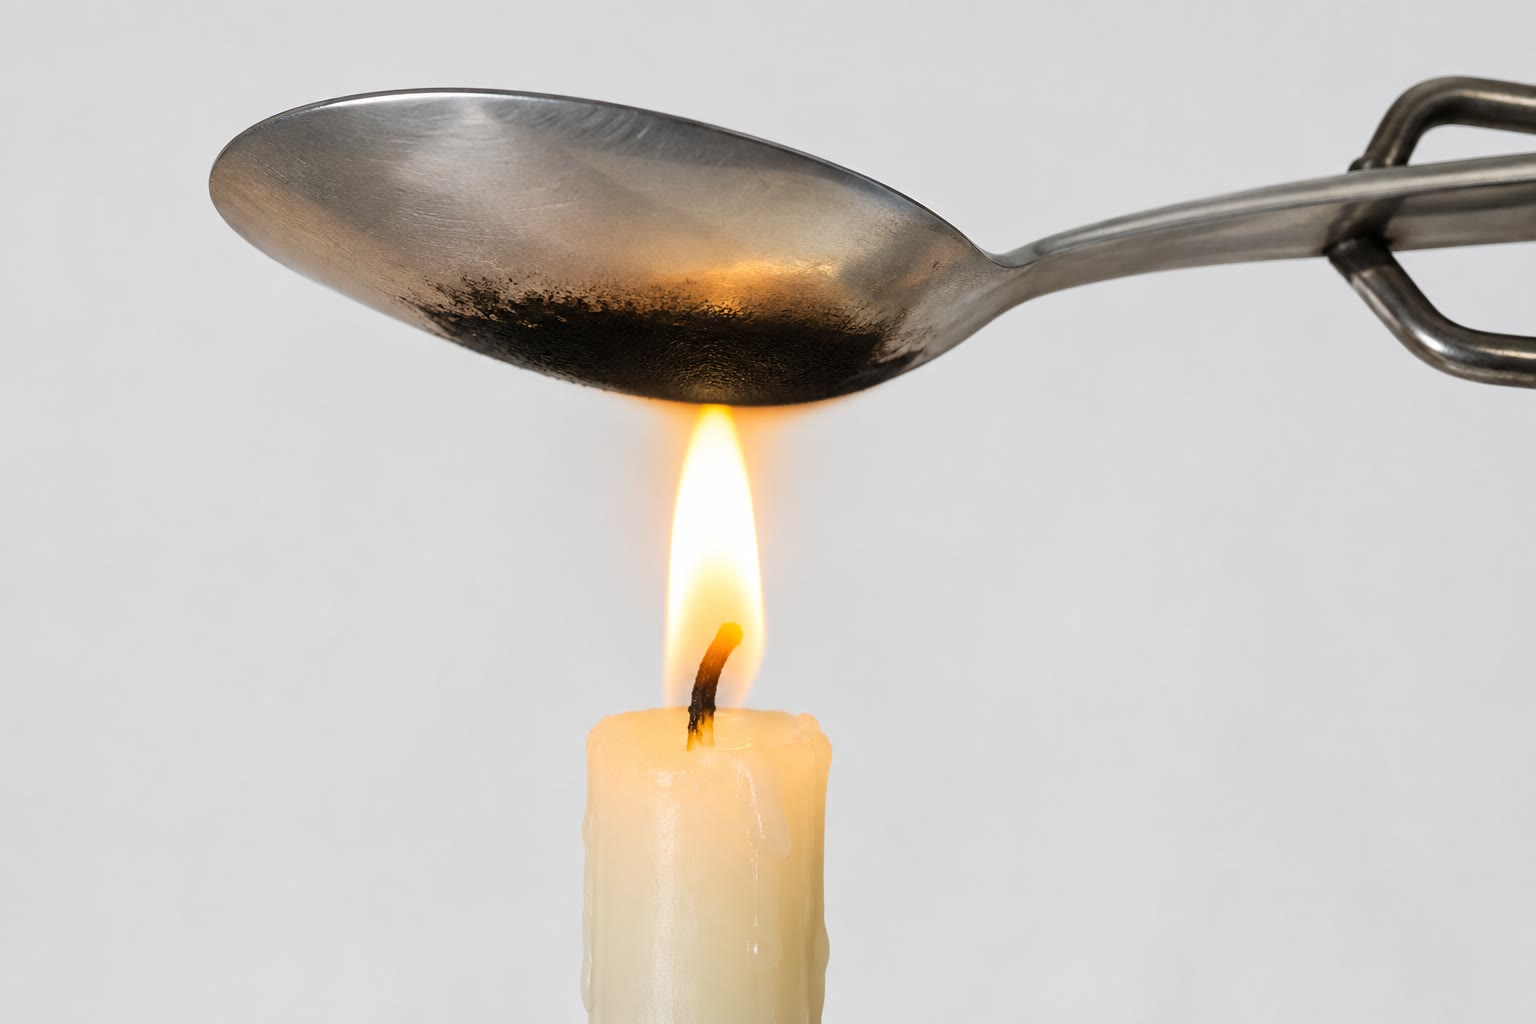
\includegraphics[width=0.45\linewidth]{images/book1/ai/g8-soot-spoon.jpg}

{\small ملعقة باردة تُمسك في لهب شمعة أصفر يسوّدها السخام: \omterm{def:g8:combustion-and-fuels:complete}{فالاحتراق
غير تام}.}
\end{omfigure}

\section{أول أكسيد الكربون، خطر صامت}

\begin{proposition}[لماذا يقتل أول أكسيد الكربون]\label{prop:g8:combustion-and-fuels:co}
أول أكسيد الكربون لا لون له ولا رائحة ولا طعم. فإذا استُنشق حلّ محل
الأكسجين في الدم (ويشرح كتاب الأحياء كيف)، فيسبب الصداع والنعاس، وفي
الغرفة المغلقة فقدان الوعي والموت. ويصنعه كل \omterm{def:g4:what-a-fire-needs:fuel}{وقود} يحترق وينقصه \omterm{def:g4:air-a-mixture-of-gases:air}{الهواء}:
سخّان غاز أو سخّان ماء سيئ الصيانة أو مسدود المدخنة، أو موقد في خيمة
مغلقة، أو شواية أو مولّد كهرباء يُستعمل داخل البيت.
\end{proposition}

\begin{safety}{\ghs[0.8cm]{GHS02}\ghs[0.8cm]{GHS04}\ghs[0.8cm]{GHS06}\ghs[0.8cm]{GHS08}}
% ledger: ghs:CO
أول أكسيد الكربون: غاز شديد القابلية للاشتعال (GHS02)، يُورَّد تحت الضغط
(GHS04)؛ سام إذا استُنشق (GHS06)؛ يُتلف الأعضاء بالتعرض المتكرر وقد
يضر بالجنين (GHS08).
\end{safety}

\begin{remark}[الوقاية من التسمم]\label{rem:g8:combustion-and-fuels:prevent}
يتعهد أجهزةَ الغاز فنيٌّ مختص بالصيانة بانتظام، ولا تُسد المداخن وفتحات
التهوية أبدًا، ولا تُستعمل الشوايات ومولّدات الكهرباء إلا في الخارج، ويُركّب
جهاز إنذار لأول أكسيد الكربون قرب كل موقد.
\end{remark}

\begin{omfigure}
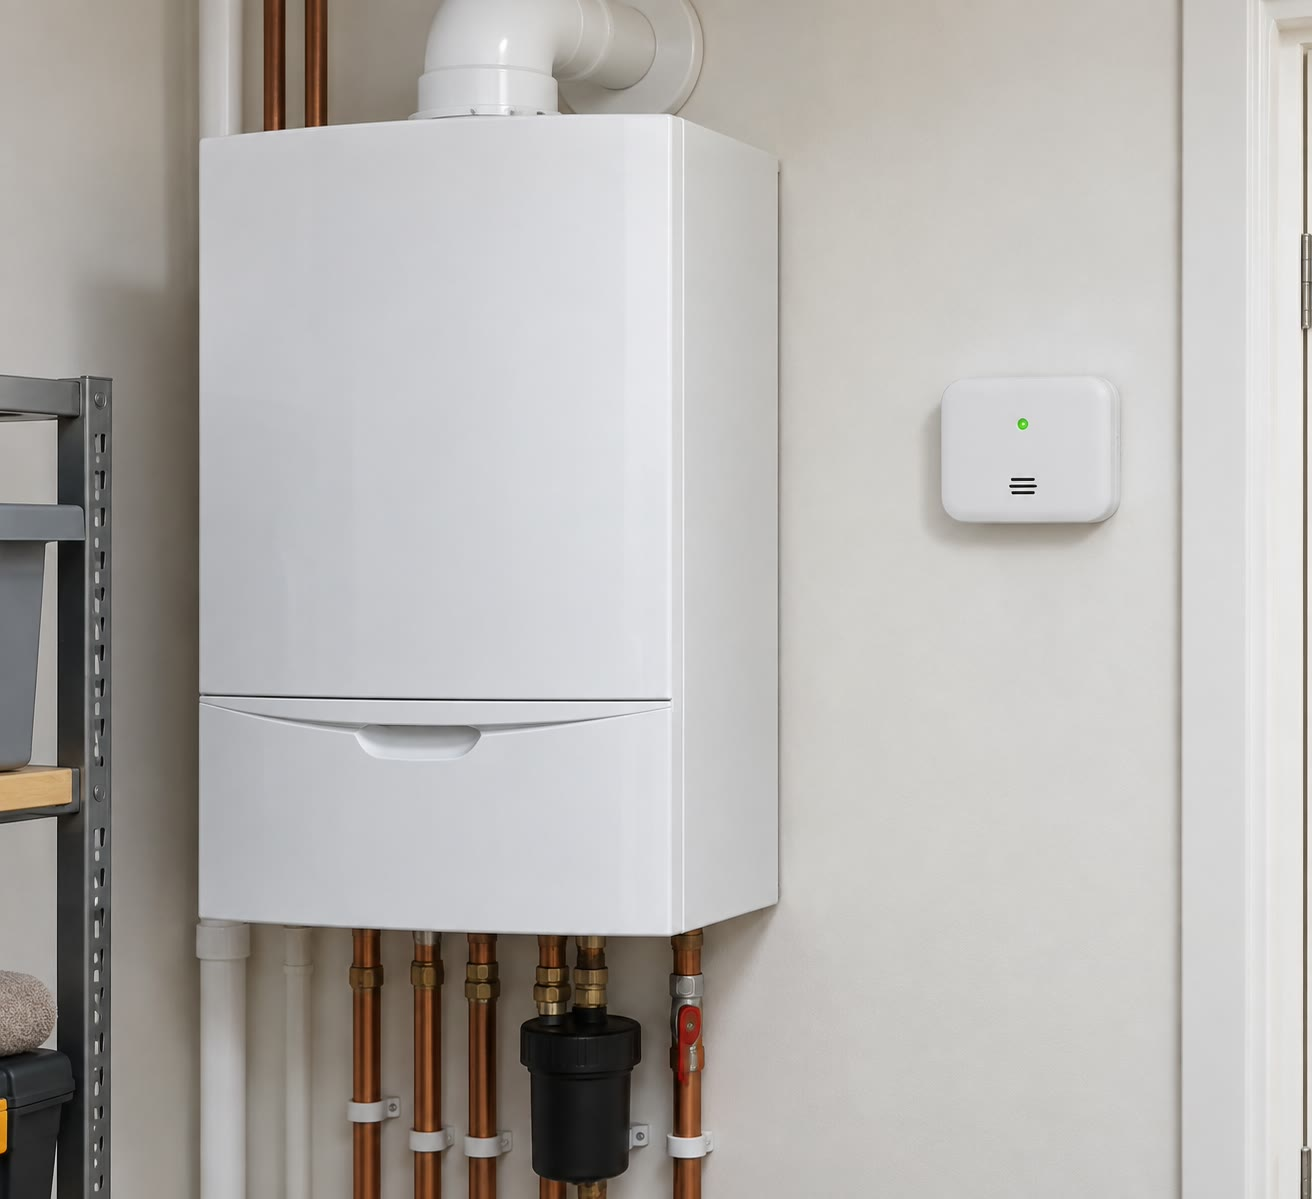
\includegraphics[width=0.45\linewidth]{images/book1/ai/g8-boiler-alarm.jpg}

{\small سخّان غاز، وبجانبه جهاز إنذار لأول أكسيد الكربون.}
\end{omfigure}

\section{ثنائي أكسيد الكربون وظاهرة الدفيئة}

\begin{definition}[غاز الدفيئة]\label{def:g8:combustion-and-fuels:greenhouse}
\emph{غاز الدفيئة}\index{غاز دفيئة} غاز من غازات \omterm{def:g4:air-a-mixture-of-gases:air}{الهواء} يسمح بمرور ضوء
الشمس لكنه يحبس جزءًا من الحرارة التي يرسلها سطح الأرض نحو الفضاء، فيدفّئ
الطبقات السفلى من الغلاف الجوي. فبخار الماء وثنائي أكسيد الكربون والميثان
غازات دفيئة؛ أما النيتروجين والأكسجين فلا. (ويشرح كتاب الفيزياء كيف يحدث
ذلك.)
\end{definition}

\begin{proposition}[ثنائي أكسيد الكربون في الهواء في ازدياد]\label{prop:g8:combustion-and-fuels:rising}
% ledger: co2:mlo-1959, co2:mlo-2025 (rise 111.4 ppm, +35 %)
يُقاس مقدار ثنائي أكسيد الكربون في \omterm{def:g4:air-a-mixture-of-gases:air}{الهواء} دون انقطاع منذ 1959 في مرصد على
جبل وسط المحيط الهادئ. فقد كان 316 جزءًا في المليون (ppm) من \omterm{def:g4:air-a-mixture-of-gases:air}{الهواء} سنة
1959 و427 ppm سنة 2025: أي ارتفع بنحو \qty{35}{\percent} في عمر إنسان
واحد، وذلك في معظمه من حرق الفحم والنفط والغاز الطبيعي. وثنائي أكسيد
الكربون الزائد يقوّي ظاهرة الدفيئة ويدفّئ المناخ.
\end{proposition}

\begin{omfigure}
\begin{tikzpicture}
\begin{axis}[width=0.85\linewidth, height=6cm, xmin=1955, xmax=2030,
    ymin=300, ymax=440, xlabel={السنة}, ylabel={\foreignlanguage{arabic}{ثنائي أكسيد الكربون \babelsublr{(ppm)}}},
    axis lines*=left, ymajorgrids, grid style={gray!20},
    tick label style={font=\small, /pgf/number format/1000 sep={}},
    label style={font=\small}]
\addplot[omDef, thick, mark=*, mark size=0.8pt]
  table[x=year, y=ppm] {figdata/out/grade-8-co2-record.dat};
\node[anchor=west, font=\small] at (axis cs:1962,306) {\foreignlanguage{arabic}{\babelsublr{316} \babelsublr{ppm} سنة \babelsublr{1959}}};
\node[anchor=east, font=\small] at (axis cs:2023,428) {\foreignlanguage{arabic}{\babelsublr{427} \babelsublr{ppm} سنة \babelsublr{2025}}};
\end{axis}
\end{tikzpicture}

{\small المتوسط السنوي لثنائي أكسيد الكربون في \omterm{def:g4:air-a-mixture-of-gases:air}{الهواء}، مقيسًا منذ 1959
(بيانات مختبر الرصد العالمي التابع للإدارة الوطنية للمحيطات والغلاف الجوي؛
وقبل 1974، معهد سكريبس لعلوم المحيطات).}
\end{omfigure}

\section{الوقود الأحفوري والوقود المتجدد}

\begin{definition}[الوقود الأحفوري والوقود المتجدد]\label{def:g8:combustion-and-fuels:fossil}
\emph{الوقود الأحفوري}\index{وقود أحفوري} --- الفحم الحجري، والنفط،
والغاز الطبيعي --- تكوّن تحت الأرض على مدى ملايين السنين من بقايا نباتات
وكائنات بحرية قديمة. أما \emph{الوقود المتجدد}\index{وقود متجدد} فيُصنع
من نباتات تُزرع اليوم، أو من النفايات: الخشب، والغاز الحيوي من السماد
الحيواني وبقايا الطعام، والإيثانول المصنوع من الشمندر السكري أو قصب السكر.
\end{definition}

\begin{proposition}[من أين يأتي الكربون]\label{prop:g8:combustion-and-fuels:cycle}
تأخذ النباتات ثنائي أكسيد الكربون من \omterm{def:g4:air-a-mixture-of-gases:air}{الهواء} لتنمو. وحرق \omterm{def:g8:combustion-and-fuels:fossil}{الوقود المتجدد}
يعيد ثنائي أكسيد الكربون الذي أخذته نباتاته من \omterm{def:g4:air-a-mixture-of-gases:air}{الهواء} قبل بضع سنوات. أما
حرق \omterm{def:g8:combustion-and-fuels:fossil}{الوقود الأحفوري} فيطلق كربونًا كان محبوسًا تحت الأرض ملايين السنين:
فهو يضيف ثنائي أكسيد الكربون إلى \omterm{def:g4:air-a-mixture-of-gases:air}{الهواء}.
\end{proposition}

\begin{omfigure}
\begin{tikzpicture}[font=\small,
    box/.style={draw=omDef, fill=omDef!6, rounded corners=2pt, align=center,
      minimum height=0.9cm, text width=2.6cm}]
  \node[box] (air) at (0,3) {ثنائي أكسيد الكربون\\ في الهواء};
  \node[box] (plants) at (5.6,3) {النباتات تنمو\\ (\foreignlanguage{arabic}{تأخذ \ce{CO2}})};
  \node[box] (fuel) at (5.6,0.4) {خشب، غاز حيوي،\\ إيثانول حيوي};
  \node[box, draw=black!50, fill=black!8] (fossil) at (0,0.4) {فحم، نفط، غاز:\\ تحت الأرض};
  \draw[->, thick, omProp] (air) -- (plants);
  \draw[->, thick, omProp] (plants) -- (fuel);
  \draw[->, thick, omProp] (fuel) -- (air);
  \node[text=black, font=\footnotesize, align=left, anchor=north west] at (1.5,1.45)
    {الحرق،\\ بعد بضع سنوات};
  \draw[->, thick, black!60] (fossil) -- node[midway, left, text=black, font=\footnotesize,
    align=right] {الحرق:\\ كربون مخزّن\\ منذ ملايين\\ السنين} (air);
\end{tikzpicture}

{\small \omterm{def:g8:combustion-and-fuels:fossil}{الوقود المتجدد} يعيد إلى \omterm{def:g4:air-a-mixture-of-gases:air}{الهواء} الكربون الذي أخذته نباتاته منه؛
\omterm{def:g8:combustion-and-fuels:fossil}{والوقود الأحفوري} يضيف كربونًا كان مخزّنًا تحت الأرض.}
\end{omfigure}

\begin{omfigure}
\begin{minipage}[t]{0.48\linewidth}\centering
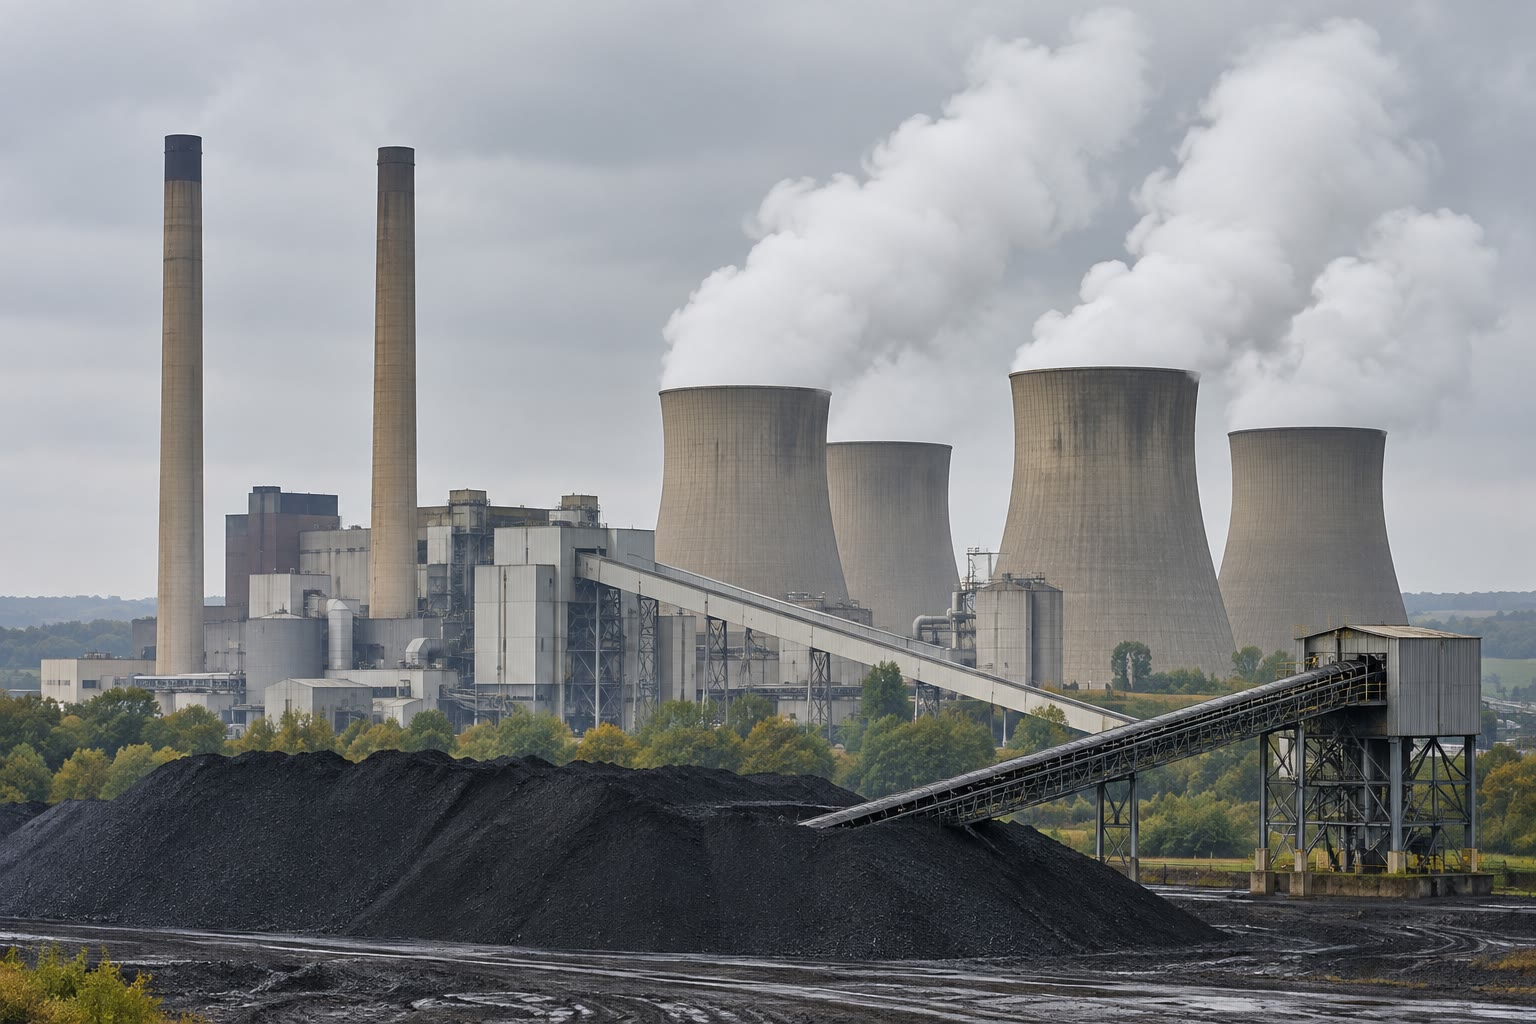
\includegraphics[width=\linewidth,height=4.6cm,keepaspectratio]{images/book1/ai/g8-coal-plant.jpg}

{\small محطة كهرباء تعمل بالفحم.}
\end{minipage}\hfill
\begin{minipage}[t]{0.48\linewidth}\centering
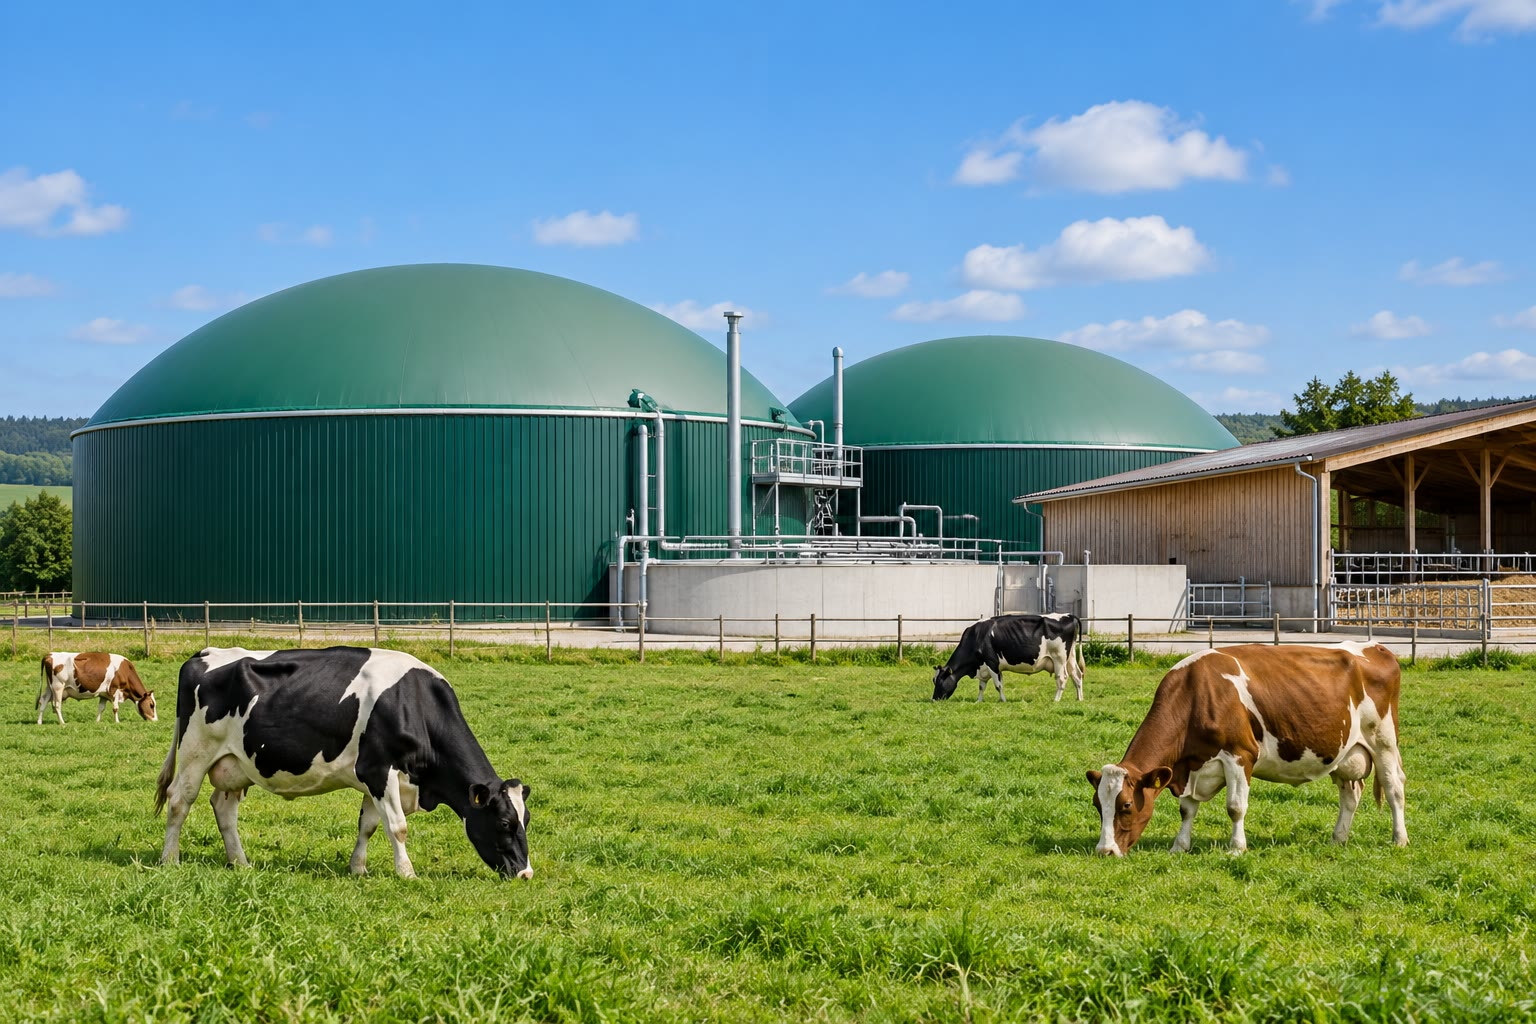
\includegraphics[width=\linewidth,height=4.6cm,keepaspectratio]{images/book1/ai/g8-biogas-farm.jpg}

{\small محطة غاز حيوي في مزرعة: السماد الحيواني يصير وقودًا متجددًا.}
\end{minipage}
\end{omfigure}

\section{تمارين}

\begin{exercise}[$\star$]\label{exo:g8:combustion-and-fuels:1}
اكتب \omterm{def:g8:balanced-equations:equation}{المعادلة الموزونة} \omterm{def:g8:combustion-and-fuels:complete}{للاحتراق التام} للكربون.
\end{exercise}

\begin{exercise}[$\star$]\label{exo:g8:combustion-and-fuels:2}
ما الفرق بين \omterm{def:g8:combustion-and-fuels:complete}{الاحتراق التام} \omterm{def:g8:combustion-and-fuels:complete}{والاحتراق غير التام}؟
\end{exercise}

\begin{exercise}[$\star$]\label{exo:g8:combustion-and-fuels:3}
لماذا يُسمى أول أكسيد الكربون خطرًا صامتًا؟
\end{exercise}

\begin{exercise}[$\star$]\label{exo:g8:combustion-and-fuels:4}
أحفوري أم متجدد: الفحم، والخشب، والغاز الطبيعي، والغاز الحيوي، والبنزين،
والإيثانول المصنوع من الشمندر السكري؟
\end{exercise}

\begin{exercise}[$\star\star$]\label{exo:g8:combustion-and-fuels:5}
اكتب \omterm{def:g8:balanced-equations:equation}{المعادلة الموزونة} \omterm{def:g8:combustion-and-fuels:complete}{للاحتراق التام} للبروبان،
\ce{C3H8}.
\end{exercise}

\begin{exercise}[$\star\star$]\label{exo:g8:combustion-and-fuels:6}
يحترق الإيثانول، \ce{C2H6O}، \omterm{def:g4:what-a-fire-needs:burning}{احتراقًا} تامًا في الأكسجين. وازن
\ce{C2H6O + O2 -> CO2 + H2O}. % ce-unbalanced-ok (to balance)
\end{exercise}

\begin{exercise}[$\star\star$]\label{exo:g8:combustion-and-fuels:7}
مقلاة تُمسك فوق لهب أصفر يسودّ أسفلها. ما المادة السوداء؟ وماذا تخبرنا
عن \omterm{def:g4:what-a-fire-needs:burning}{الاحتراق}؟
\end{exercise}

\begin{exercise}[$\star\star$]\label{exo:g8:combustion-and-fuels:8}
اقرأ منحنى ثنائي أكسيد الكربون: كم كان في \omterm{def:g4:air-a-mixture-of-gases:air}{الهواء} من ثنائي أكسيد الكربون
تقريبًا سنة 1980 وسنة 2000؟ وبكم ppm ارتفع في هذه السنوات
العشرين؟
\end{exercise}

\begin{exercise}[$\star\star$]\label{exo:g8:combustion-and-fuels:9}
لماذا يضيف حرق الخشب إلى \omterm{def:g4:air-a-mixture-of-gases:air}{الهواء}، على مر السنين، ثنائي أكسيد كربون أقل مما
يضيفه حرق الفحم، مع أن كليهما يعطي ثنائي أكسيد الكربون؟
\end{exercise}

\begin{exercise}[$\star\star$]\label{exo:g8:combustion-and-fuels:10}
وازن \omterm{def:g8:combustion-and-fuels:complete}{الاحتراق غير التام} للكربون إلى أول أكسيد الكربون،
\ce{C + O2 -> CO}. % ce-unbalanced-ok (to balance)
\end{exercise}

\begin{exercise}[$\star\star\star$]\label{exo:g8:combustion-and-fuels:11}
من 1959 (316 ppm) إلى 2025 (427 ppm)، بأي نسبة مئوية ازداد ثنائي أكسيد
الكربون في \omterm{def:g4:air-a-mixture-of-gases:air}{الهواء}؟ قرّب إلى أقرب عدد صحيح.
\end{exercise}

\begin{exercise}[$\star\star\star$]\label{exo:g8:combustion-and-fuels:12}
تُستعمل مدفأة غاز في غرفة صغيرة نافذتها مغلقة. اشرح، مستعملًا معادلتين من هذا
الفصل، كيف يمكن أن يتحول \omterm{def:g4:what-a-fire-needs:burning}{الاحتراق} من تام إلى غير تام مع مرور الوقت، ولماذا
يكون ذلك خطرًا.
\end{exercise}

\section{مسألة: الموقد في الخيمة}

\begin{problem}[{مسألة نهاية الأسبوع --- موقد تخييم، والغاز الذي يحرقه،
وما يصنعه، ولماذا لا يدخل الخيمة أبدًا}]
\label{pb:g8:combustion-and-fuels:1}
% ledger: ghs:propane
يحرق موقد تخييم البروبان، \ce{C3H8}، من عبوة تحوي
\qty{450}{g} منه. وفي \omterm{def:g4:air-a-mixture-of-gases:air}{الهواء} الطلق يكون اللهب أزرق. خذ نسب الكتل هذه،
المستخرجة من \omterm{def:g8:balanced-equations:equation}{المعادلة الموزونة}: \qty{44}{g} من البروبان المحترق \omterm{def:g4:what-a-fire-needs:burning}{احتراقًا}
تامًا تعطي \qty{132}{g} من ثنائي أكسيد الكربون.

\medskip
\noindent\textbf{الجزء الأول --- المعادلات.}
\begin{enumerate}
  \item اكتب \omterm{def:g8:balanced-equations:equation}{المعادلة الموزونة} \omterm{def:g8:combustion-and-fuels:complete}{للاحتراق التام}
        للبروبان.
  \item تحقق منها بعدّ \omterm{def:g7:atoms-and-molecules:atom}{الذرات} من كل نوع في كل طرف.
  \item وازن \omterm{def:g8:combustion-and-fuels:complete}{الاحتراق غير التام}
        \ce{C3H8 + O2 -> CO + H2O}. % ce-unbalanced-ok (to balance)
  \item أي الاحتراقين يحتاج إلى أكسجين أكثر لكل \omterm{def:g7:atoms-and-molecules:molecule}{جزيء} بروبان؟
\end{enumerate}

\medskip
\noindent\textbf{الجزء الثاني --- داخل الخيمة.}
\begin{enumerate}[resume]
  \item موقد يُشعل داخل خيمة مغلقة سرعان ما يحترق بلهب أصفر.
        علّل.
  \item أي غاز خطر يتكوّن عندئذ؟ اذكر خاصيتين من خصائصه تجعلان
        الانتباه إليه صعبًا.
  \item تحمل عبوة البروبان رمزي خطر. سمّهما وقل
        ما يعنيه كل منهما.
  \item اذكر قاعدتين لاستعمال موقد التخييم بأمان.
\end{enumerate}

\medskip
\noindent\textbf{الجزء الثالث --- ثنائي أكسيد الكربون من عبوة واحدة.}
\begin{enumerate}[resume]
  \item كم مرة يزيد ثنائي أكسيد الكربون المتكوّن ثقلًا على البروبان
        المحترق؟
  \item من أين تأتي الغرامات الزائدة؟
  \item هل البروبان \omterm{def:g8:combustion-and-fuels:fossil}{وقود أحفوري} أم \omterm{def:g8:combustion-and-fuels:fossil}{وقود متجدد}؟ وهل يضيف حرقه ثنائي
        أكسيد الكربون إلى \omterm{def:g4:air-a-mixture-of-gases:air}{الهواء}؟
  \item احسب كتلة ثنائي أكسيد الكربون المنطلقة حين تحترق عبوة كاملة من
        \qty{450}{g} \omterm{def:g4:what-a-fire-needs:burning}{احتراقًا} تامًا.
\end{enumerate}
\end{problem}
